\documentclass{sig-alternate}


\usepackage{graphicx}
\usepackage{amssymb}
\usepackage{epstopdf}
\usepackage{algorithmic}
\DeclareGraphicsRule{.tif}{png}{.png}{`convert #1 `dirname #1`/`basename #1 .tif`.png}

\conferenceinfo{SIGMOD}{'10 Indianapolis, IN}

\title{Streamlining Data Warehousing through Compilation}
\numberofauthors{3}
\author{}%Oliver Kennedy, Yanif Ahmad, Christoph Koch}
%\date{}                                           % Activate to display a given date or no date

\toappear{}

\newtheorem{example}{Example}

\begin{document}

\maketitle
%\section{}
%\subsection{}

\abstract{
Performing analytics on corporate relational data is difficult; Transactional relational databases optimized for small, frequent updates, are ill suited for the aggregate-heavy demands of online analytics workloads.  Datacubes and similar datastructures are better suited to dealing with such workloads, but create an update bottleneck, as even incremental cube update techniques are too slow to avoid batching.  In this paper, we sidestep the issue of constructing and maintaining datacubes cube updates with the SpreadDB\footnote{The name ``SpreadDB" is anonymized for double-blind reviewing} system.  SpreadDB aggressively compiles datacube construction queries into to a distributed, main-memory data warehouse runtime.  Incremental update rules generated by SpreadDB's compiler make it possible to dynamically make the data warehouse mirror a corporate relational database in near-real-time.  Combining low-delay synchronization with purely in-memory data storage makes it possible to evaluate OLAP queries on large, \textit{live} datasets in a matter of seconds, rather than minutes or hours.
}
\section{Introduction}

Consider a typical corporate datacube infrastructure.  At one end, lie one or more OLTP databases.  These databases manage corporate data in a standard relational infrastructure that permit easy updates to minor components.  However, for read-heavy, non-transactional analytics workloads, this infrastructure is insufficient.  Conversely, datacubes\cite{datacube} excel at analytics workloads, but do not support transactional relational updates.  Corporations that require heavy-duty analysis of relational data often resort to periodically extracting the contents of their relational database to reconstruct or update their analytics datastructures, a process that can take hours, or even days.

Periodic scraping is inefficient.  Not only does each run duplicate effort expended by prior runs, the time spent reconstructing (or even only updating) an entire datacube ensures that analysts are working with stale versions of the data.  

In this paper, we present SpreadDB, a system that constructs and maintains an in-memory OLAP database in near-real time.  SpreadDB is developed based on three observations about current corporate datacube infrastructures:
\begin{enumerate}
\item Disk drive sizes are dramatically larger than they were a few years ago, but disk read latency remains nearly constant\cite{}; To minimize latency, disk-based corporate datacubes and other analytics structures are stored on vastly more (nearly empty) disks than are requried.\cite{}
\item RAM is cheap, plentiful, and low-latency; Server-class machines commonly have 32 GB of ram apiece\cite{}.  Terrabyte ram DIMMs are becoming available\cite{}
\item Aggregation is a highly parallelizable task.
\end{enumerate}

Rather than maintaining a datacube partitioned across an array of disks, SpreadDB constructs the entire datacube in-memory across a network of machines.  The minimal functionality required from each node in this network not only minimizes the cost of those nodes, but allows them to be constructed without the use of error-prone, temperature-sensitive disk drives.  

Because all state is stored in-memory rather than on-disk, SpreadDB is amenable to the use of non-linear datastructures, for example datacubes.  Moreover, because data is partitioned, the task of projecting and aggregating is be easily farmed out to the hosting nodes.  Using a set of novel compilation and optimization techniques, SpreadDB translates datacube construction queries into an entire data warehouse infrastructure.  

SpreadDB's compiler produces an aggressively optimized execution plan that translates updates to the individual tables of an underlying relational database updates into delta operations on the warehouse.  Additionally, the compiler generates a \textit{distribution plan} that guides data partitioning across nodes within the warehouse to maximize communication efficiency.  The result is a warehouse infrastructure that not only answers OLAP queries quickly and efficiently, but that can use live data to answer those queries.

\begin{example}\textit
As a running example in this paper, we will use a datacube loosely based on TPC-H\cite{tpch} Query 12:
\end{example}
\begin{figure}
\begin{center}
\textbf{Schema}
\end{center}
\begin{algorithmic}
\STATE \textbf{create table} customers(cid \textit{int}, nid \textit{int}); 
\STATE \textbf{create table} orders(
\STATE \hspace*{0.1in} oid \textit{int}, o\_cid \textit{int}, opriority \textit{int}, spriority \textit{int},
\STATE \hspace*{0.1in}  \textbf{foreign key}(o\_cid) \textbf{references} customers(oid)
\STATE );
\STATE \textbf{create table} lineitems(
\STATE \hspace*{0.1in} l\_oid \textit{int}, lateship \textit{int}, latecommit \textit{bool}, shipmode \textit{bool},
\STATE \hspace*{0.1in} \textbf{foreign key}(l\_oid) \textbf{references} orders(oid)
\STATE );
\end{algorithmic}
\begin{center}
\textbf{Query}
\end{center}
\begin{algorithmic}
\STATE \textbf{select} count(*),
\STATE \hspace*{0.1in} nid, cid, oid, opriority, spriority, 
\STATE \hspace*{0.1in} lateship, latecommit, shipmode 
\STATE \textbf{from} customers, orders, lineitems 
\STATE \textbf{where} o\_cid=cid and l\_oid=oid 
\STATE \textbf{group by cube} 
\STATE \hspace*{0.1in} nid, cid, oid, opriority, spriority, 
\STATE \hspace*{0.1in} lateship, latecommit, shipmode;
\end{algorithmic}
\caption{An example query that constructs a warehouse for analyzing customer behavior with respect to shipping.  Given a table of customers, orders, and lineitems in those orders, the query builds a datacube over the full join of those tables.}
\label{fig:example}  
\end{figure}

\section{Architecture}
\label{sec:architecture}
\begin{figure}
\begin{center}
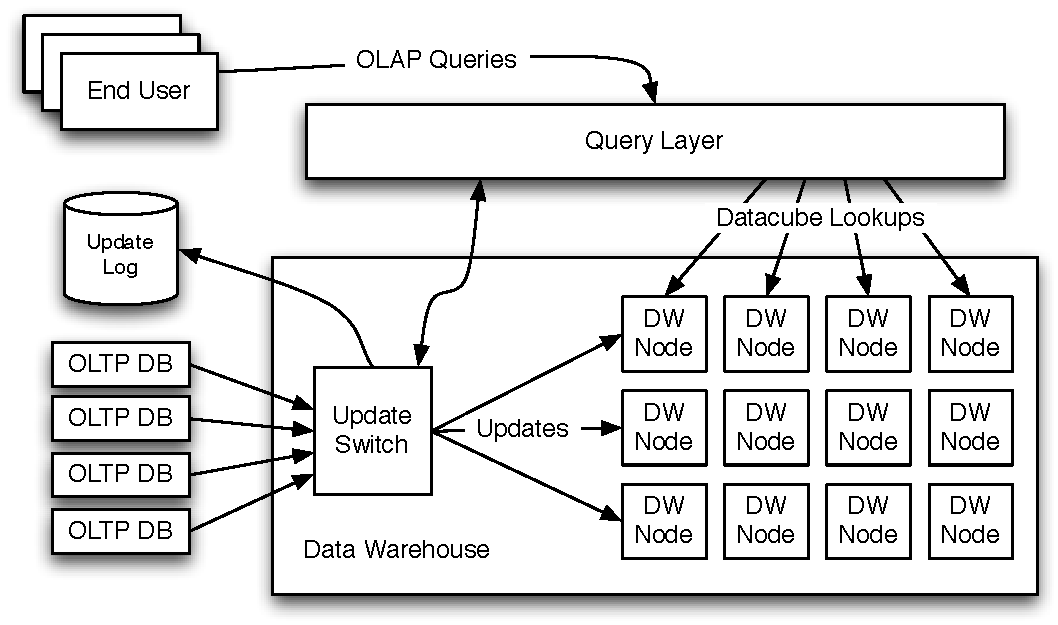
\includegraphics[width=3in]{images/Architecture.pdf}
\caption{SperadDB's architecture.}
\label{fig:arch}
\end{center}
\end{figure}
SpreadDB consists of three components: a runtime, a \textit{Query Layer}, and a compiler.  A diagram of this architecture is presented in Figure \ref{fig:arch}.  The warehousing runtime accepts relation updates at a coordinator node called the \textit{Switch}, and distributes their data throughout an array of data warehouse storage nodes, or \textit{DW Nodes}.  Though this paper focuses on a runtime with a centralized switch, we discuss a distributed switch implementation in Section \ref{sec:distswitch}.

Adjacent to the runtime is the \textit{Query Layer}, a component that acts as an intermediary between the end user and the dw nodes.  The query layer accepts roll-up and drill-down queries, translates them into the corresponding set of data warehouse lookups, and executes those queries on the warehouse.

SpreadDB's final component is a compiler that guides the behavior of the other three components.  Given an arbitrary SQL query, the SpreadDB compiler produces a set of update rules, or \textit{Triggers}.  Each trigger is invoked at the Switch when one of the query's input tables is modified, and begins the process of applying the appropriate changes within the warehouse.  

Changes applied by a trigger are a form of delta-encoding.  SpreadDB maintains a set of \textit{Maps} on the DW Nodes to minimize the work required to process any individual update to an input table.  Every trigger incrementally updates the appropriate map, potentially using data from other maps.  The compilation and construction of triggers is discussed in further detail in Section \ref{sec:compilation}.  In short, every trigger consists of one or more \textit{Map Update Rules} that take the following form:
$$+R(Params)\ :\ Map[Key, Key, \ldots]\ += Expression$$
Here, the Trigger is fired when the tuple $(Params)$ is inserted into Table $R$.  When this happens, the target $Map$ is modified by the corresponding algebraic $Expression$ of constants, references to other maps, and variables bound to the input parameters.  Map references are indexed by one or more $Key$s, which may be constants or variables, but not references to other maps.  Thus, the total latency for expression evaluation on a quiescent system is limited to at most two network hops.  

Finally, some Update Rules may modify an entire cross section of a map.  Such updates are expressed via unbound variables in the update rule-that is, variables not bound to one of the input parameters.  These loop parameters occur both as a target key and within the update expression.  Update rules behave as if they were a set of parallel updates; every update in the set corresponds to one valuation of all loop variables selected from their contextually identified domains.  

\subsection{Anatomy of an Update}

\begin{figure}
\begin{center}
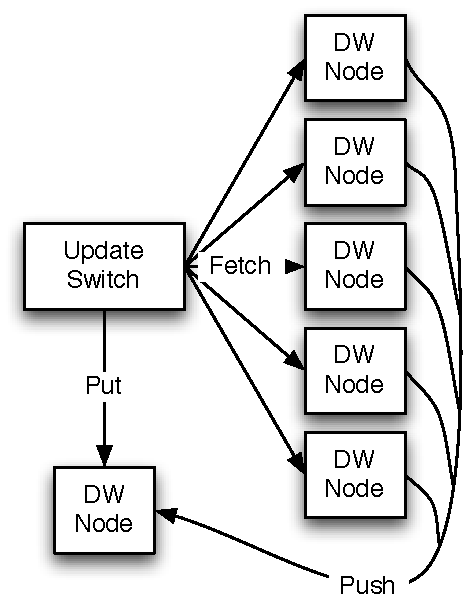
\includegraphics[width=1.5in]{images/UpdateStep.pdf}
\caption{Information flow during one map update.}
\label{fig:updatestep}
\end{center}
\end{figure}

A map update begins at the Switch when an input table is modified.  Each input table is associated with one or more triggers, each requiring a write to some range of map values and zero or more reads from different maps.  For each trigger, the Switch identifies and sends a PUT message to each DW Node managing a map being written to.  Additionally, the Switch identifies all DW Nodes managing maps that will be read from and sends a FETCH message to them, requesting the desired map values.  Finally, if required (i.e., if SpreadDB is being used standalone, without an underlying database), the switch can log the update to disk for persistence.

The nodes receiving a FETCH request perform the appropriate reads and send their responses to the PUT nodes in a PUSH message.  Upon receipt of all necessary PUSH messages, the PUT nodes compute the update expression and modify the affected maps.  An illustration of the complete message-passing process is presented in Figure \ref{fig:updatestep}.  

\subsubsection{Trigger Dispatch}
Maps are partitioned along dimensional axes when they grow beyond the capacity of a single node, akin to the partitioning done in grid files\cite{318586}.  To streamline the dispatch of messages to component nodes, the switch pre-generates a spatial index for each template, similar to the grid file directory.  Every entry in the spatial index contains a set of PUT and FETCH messages.  When the template is triggered, the tuple's values are used to index into the spatial index and the corresponding messages are parametrized and sent.  The algorithm for generating the spatial index is presented in Figure \ref{alg:dispatch}.

\begin{figure}
\begin{algorithmic}[1]
\STATE $Msgs \leftarrow \emptyset$
\FORALL{Update $U \in$ Trigger}
	\STATE Region $Reg = \pi_{U.target.loop\_vars} \left(index(U.target\_map)\right)$
	\FORALL{Partition $\{P | P\in U.target\_map \wedge (P \cap Reg \neq \emptyset)\}$}
		\STATE $Reads = \emptyset$
		\FORALL{Ref $R \in get\_map\_refs(U.expression)$}
			\STATE $RReg \leftarrow \pi_{R.loop\_vars} P$
			\STATE $RPart \leftarrow \{RP | RP\in R.map \wedge (RP \cap RReg \neq \emptyset)\}$
			\STATE $Reads \leftarrow Reads \cup \{(ReadP.node, R)\}$
		\ENDFOR
		\STATE $Reads \leftarrow group\_by\_node(Reads)$
		\STATE $Msgs \leftarrow put(U, P, Reads.size)$
		\FORALL{$($Node $N, \{$Ref $R\}) \in Reads$}
		  \STATE // PUSH results to $P.node$
			\STATE $Msgs \leftarrow fetch(N, \{R\}, P.node)$
		\ENDFOR
	\ENDFOR
\ENDFOR
\end{algorithmic}
\caption{The Switch's trigger dispatch algorithm}
\label{alg:dispatch}
\end{figure}

Looping updates require the Switch to match corresponding read and write partitions.  The correspondence is obtained by identifying intersections between partitions of the target map that are affected by the update, and those of each map in the update expression.  This is equivalent to a join over components of the spatial index stored at the Switch.  Loop-free updates are a special case of this, where only one partition is required from each map.  The trigger dispatch algorithm is shown in Figure \ref{alg:dispatch}.

\subsubsection{Get Collation}

FETCH responses, or PUSH messages for an update are sent to the node managing the partition being updated.  Having received the number of FETCH messages sent by the switch with the PUT message, the destination node can buffer PUSH messages until all have arrived.  At this point, if the update is loop-free, the destination node simply uses the contents of the PUSH messages to evaluate the update expression.

\begin{figure}
\begin{algorithmic}[1]
\STATE Given: Update $U$
\FORALL{Ref $R \in U.expression$}
	\STATE $Inputs \leftarrow Inputs \cup (R, \emptyset)$
\ENDFOR
\FORALL{$($Ref $InR,$ Value $V) \in \cup(msg_{PUSH})$}
	\FORALL{$(R, Table) \in Inputs$}
		\IF{$check\_match(InR, R)$}
			\STATE $Table \leftarrow Table \cup (InR.keys, V)$
		\ENDIF
	\ENDFOR
\ENDFOR
\FORALL{$(K,\{V\}) \in $ JOIN $ (Keys, Val) \in Inputs$}
	\STATE $Target = bind\_vars(U.target \leftarrow Keys)$
	\STATE $apply(Target, bind\_vars(U.expression \leftarrow \{V\}))$
\ENDFOR
\end{algorithmic}
\caption{The DW Node's collation algorithm}
\label{alg:collation}
\end{figure}

If the update requires a loop, the destination node must do some processing.  The node first generates a set of tables, one for each map reference in the update expression.  Arriving map values populate tables that correspond to any map reference matching the value's keys, where loop variables act as wildcards.  When all values have been received, the destination node computes the natural join of all of the generated tables, effectively producing one update value for every assigned value in the domain of all of the loop variables.  The loop-free update is a special case of this where each generated table contains only one row.  The collation algorithm is shown in Figure \ref{alg:collation}

\subsection{Consistency Model}

SpreadDB's update delta-encoding uses materialize subqueries already stored within the warehouse to perform updates.  This dependency requires that all reads see a consistent snapshot of the warehouse at the completion of the previous update.  Thus, all reads and writes must be executed as if there were a total ordering over all updates.  As the clearinghouse for updates, the Switch presents an ideal point for generating this ordering.  

Every update is assigned a version number by the switch as it is issued.  The 
As they are 

Every update is assigned a version number by the switch.  The maps that each update modifies and reads are known.  The switch maintains a list of modification times for each partition in the warehouse.  With each request to the DW Nodes, the switch attaches a version 

 first looks up the most recent modification time for each get required by the update, and subsequently updates the modification times for each put required by the update.  

When applying gets, each warehouse node first ensures that it has successfully applied all requests prior to the indicated version number.  A short history of prior incarnations of each partition are also maintained in case a get arrives after a subsequent put.  Each put also includes the version number of the last fully completed update.  This allows the target node to discard old incarnations of the partition.

Some trickery will be required to get this table into the middleware.  Perhaps the switch can periodically broadcast it over?

\section{Compilation}
\label{sec:compilation}

\subsection{Update Rules}
- Translating SQL into Update Rules

- Update DAGs/Data flow graphs

- Exploiting Foreign Keys

- Cascading Map Rejection

\begin{figure}
\begin{center}
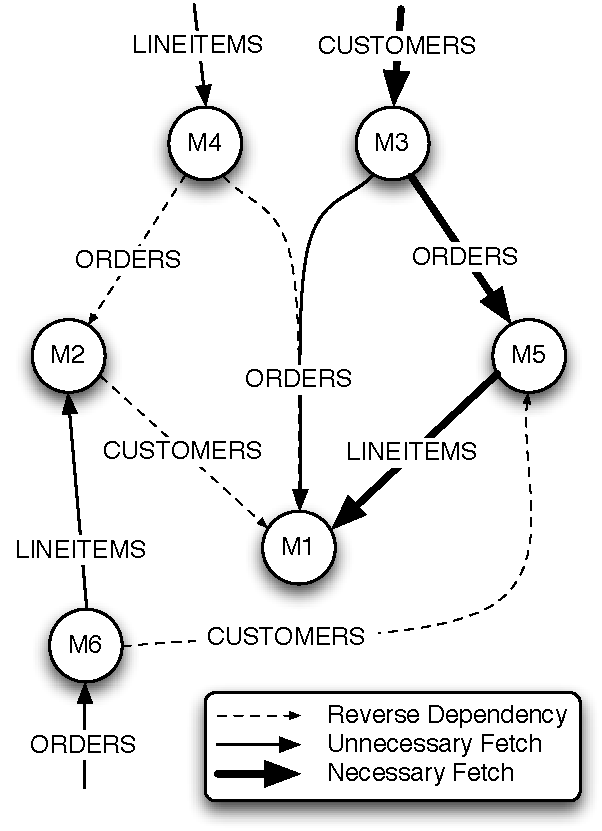
\includegraphics[width=2.5in]{images/q12_graph.pdf}
\caption{Data-flow graph for the example query.  Light and dashed edges can be optimized out, given cascading delete foreign key constraints.}
\label{fig:dataflow}
\end{center}
\end{figure}

\subsection{Layout}
How do we partition data (the layout)?  Where do various bits of code get executed live?  What kind of runtime analytics do we need to collect to manage the data layout on the fly? 

\section{Distributing the Switch}
\label{sec:distswitch}
The role of the switch is to provide a synchronization mechanism for the updates.  Specifically, the delta encoding approach used by the update rules requires that all update rules be applied to a consistent snapshot of the maps.  The current implementation of SpreadDB performs this synchronization at a single node.  However, limiting the switch to only one node creates a scaling bottleneck.  

Despite the cloud computing mantra of rejecting consistency, this application requires it.  Complex locking protocols have poor scaling performance, so a simpler, lock-free protocol is required.  We achieve this goal by introducing the notion of \textit{pipeline scheduling}.  Pipeline scheduling exploits the acyclicity of compiler-generated data-flow graphs to allow nodes to correctly interleave and process update rules with only limited network overhead and processing latency.

\subsection{Pipeline Scheduling}
Loose clock synchronization between nodes is assumed, and allows time to be partitioned into a sequence of numbered ticks, each lasting on the order of seconds.  When a set of updates is triggered, a switch node sends tentative put requests to all participating nodes.  These nodes respond with their current tick counter, and the switch forwards the maximum returned tick to all nodes.

The updates are considered to have been posted at the maximum returned tick.  However processing is deferred for a number of ticks equal to the depth of the map being updated.  The result is a data-flow process resembling a parallelized CPU pipeline.

During a given tick, all updates scheduled for processing are evaluated.  Once all updates scheduled for the tick have completed, the node responds to FETCH requests for the tick with PUSH messages.  Recall that each edge in the data flow graph represents a FETCH request for a specific update.  The difference in depth between the edge's ends is the number of ticks in advance of the PUT that the response is sent.  

For example, in Figure \ref{fig:dataflow} without removing any edges, $Depth(M1) = 2$, $Depth(M2) = 1$, and $Depth(M4) = 0$.  Updates to map $M1$ scheduled for processing during tick 4 would receive data from map $M2$ during tick 3, and from map $M1$ during tick 2.

%\subsection{Synchronizing Ticks}
%Ensuring that nodes are operating on the same tick poses two challenges.  First, the nodes must 
%
%Clock tick synchronization requires two pieces of functionality: Asserting 
%
%Loose clock tick synchronization requires two stages.  
%
%is achieved through a cascading gossip protocol.
%
%
%\subsection{Distributed Queries}
%

\section{Experiments}
\label{sec:experiments}

\bibliographystyle{abbrv}
\bibliography{spread}




%\begin{figure}
%\begin{center}
%\begin{itemize}
%\item Middleware
%\begin{itemize}
%\item Query(Query) 
%\end{itemize}
%
%\item Warehouse Nodes
%\begin{itemize}
%\item Get(\{Entry\}, Version)
%\item Fetch(\{Entry\}, Version, Destination)
%\item Push(\{(Entry, Value)\}, Version)
%\item Put(Template, \{Params\}, Version [, Fetches])
%\end{itemize}
%
%\item Switch
%\begin{itemize}
%\item update(Relation, \{Params\})
%\end{itemize}
%
%\end{itemize}
%\caption{SpreadDB's API}
%\label{fig:api}
%\end{center}
%\end{figure}

\end{document}  